\begin{figure}[H]
    \centering

\begin{tikzpicture}
\pgfplotsset{
    every axis/.style={ymin=0},
    width=0.75\textwidth,
    height=0.25\textheight,
    xtick={1, 2, 3, 4, 5, 6, 7, 8},
    y axis style/.style={
    yticklabel style=#1,
    ylabel style=#1,
    y axis line style=#1,
    ytick style=#1}}
\begin{axis}[ scale only axis, xmin=1,xmax=8, axis y line*=left, xlabel=Number of Cores, ylabel=Duration (s), y axis style=green!75!black]
    \addplot[smooth, green!75!black, mark=o, draw] 
    coordinates 
    {
        (1,916.5284999999999)
        (2,770.823)
        (3,730.158)
        (4,716.359)
        (5,697.417)
        (6,691.65)
        (7,696.311)
        (8,688.705)
    };
\end{axis}
%
\begin{axis}[ scale only axis, xmin=1,xmax=8, axis y line*=right, axis x line=none, ylabel=DEC (j), y axis style=blue]%
    \addplot[smooth, blue, mark=x] 
    coordinates 
    {
        (1,14399.399177763471)
        (2,12877.209305183253)
        (3,12509.677836630925)
        (4,12303.453831518913)
        (5,12146.320131695311)
        (6,12224.523150141764)
        (7,12228.784522192058)
        (8,12103.20580755012)
    };
\end{axis}
%
\begin{axis}[red, scale only axis, xmin=1,xmax=8, axis y line*=right, axis x line=none, ylabel=DEC per second (w)]%
\pgfplotsset{every outer y axis line/.style={xshift=2cm}, every tick/.style={xshift=2cm}, every y tick label/.style={xshift=2cm} }
    \addplot[smooth, red ,mark=+] 
    coordinates 
    {
        (1,5.105394061735848)
        (2,6.74384286208222)
        (3,7.250950943468814)
        (4,7.384421915975002)
        (5,7.645138608434484)
        (6,7.912290983091255)
        (7,7.863639612130333)
        (8,7.875402352639286)
    };
\end{axis} 

\end{tikzpicture}
    \caption{The evolution of the DEC (blue), DEC per second (red) and duration (green) as more cores are allocated to PCM on DUT 1}
    \label{fig:exp_3_dut_1_pcm_result}
\end{figure}